% Created 2021-01-24 Sun 22:49
% Intended LaTeX compiler: pdflatex
\documentclass[11pt]{article}
\usepackage[utf8]{inputenc}
\usepackage[T1]{fontenc}
\usepackage{graphicx}
\usepackage{grffile}
\usepackage{longtable}
\usepackage{wrapfig}
\usepackage{rotating}
\usepackage[normalem]{ulem}
\usepackage{amsmath}
\usepackage{textcomp}
\usepackage{amssymb}
\usepackage{capt-of}
\usepackage{hyperref}
\usepackage{minted}
\hypersetup{colorlinks=true, linkcolor=black, filecolor=red, urlcolor=blue}
\usepackage[turkish]{babel}
\author{Eren Hatırnaz}
\date{29 Nisan 2020}
\title{Yazılım Gündemi - 2020/16\\\medskip
\large 20-26 Nisan 2020}
\hypersetup{
 pdfauthor={Eren Hatırnaz},
 pdftitle={Yazılım Gündemi - 2020/16},
 pdfkeywords={},
 pdfsubject={},
 pdfcreator={Emacs 27.1 (Org mode 9.3)},
 pdflang={Turkish}}
\begin{document}

\maketitle
\tableofcontents \clearpage\shorthandoff{=}

\begin{center}
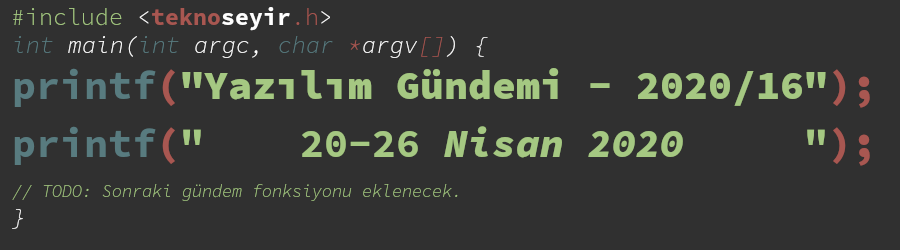
\includegraphics[width=.9\linewidth]{gorseller/yazilim-gundemi-banner.png}
\end{center}

\begin{center}
\href{../15/yazilim-gundemi-2020-15.pdf}{< Önceki Gündem} | \textbf{20-26 Nisan 2020} | \href{../17/yazilim-gundemi-2020-17.pdf}{Sonraki Gündem >}

\href{https://teknoseyir.com/blog/yazilim-gundemi-2020-16}{TeknoSeyir'de Oku}
\end{center}

\section{1 Milyon Yazılımcı \href{https://www.hurriyet.com.tr/galeri-1-milyon-yazilimci-projesi-basvurusu-nasil-yapilir-btk-akademi-egitimleri-nasil-olacak-41499705/1}{Projesi duyuruldu}}
\label{sec:orgb83a2b4}
Geçtiğimiz haftanın yazılım gündemi yazısında (bkz: \href{../15/yazilim-gundemi-2020-15.pdf}{Yazılım Gündemi - 2020/15})
Sanayi ve Teknoloji Bakanı Mustafa Varank'ın Açık Seminer etkinliğinin ilk
gününde yaptığı bazı açıklamalara yer vermiştim. Bu hafta da sırasıyla
Cumhurbaşkanı ve Hazine ve Maliye Bakanı da alanımızla ilgili bir proje
duyurdular ve bazı söylemlerle bulundular. Proje ilk "3 yılda 1 milyon
yazılımcı" gibi sloganlarla duyuruldu fakat sonrasında "1 Milyon İstihdam
Projesi" olarak güncellendi.

Proje kapsamında 'yazılımcı' olmak isteyen adaylar \href{https://1milyonistihdam.hmb.gov.tr/login}{bu adres} üzerinden kayıt
yaptırdıktan sonra BTKAkademi'nin web sitesinin "\href{https://www.btkakademi.gov.tr/portal/catalog}{Eğitim Kataloğu}" sayfasında
yer alan eğitimleri, uzaktan eğitim yoluyla takip edebilecekler. Bitirdikleri
her eğitim, "1 Milyon İstihdam Projesi" kapsamında oluşturulacak öz
geçmişlerine (CV) yetenek olarak otomatik şekilde eklenecek. Firmalar ve
kurumlar ise bu öz geçmiş havuzundaki kişilerden seçip işe alım
yapabilecekler.

Konu hakkında yorumlarımı TeknoSeyir Sosyal'de birkaç gönderi belirtsem de
eleştirilerimin politik bir yanı da olduğu için pek fazla detay vermedim. Bu
yazıda da politikadan uzak durmaya çalışarak neden bu projenin karşısında
olduğumu açıklamaya çalışacağım.

Açıkcası ben, bu projenin amacı eğitim sistemimizdeki ve sektördeki sorunları
halının altına süpürüp, insanların odaklarını farklı ve alakasız bir noktaya
çekmek olduğunu düşünüyorum. Çünkü sektörümüzdeki ve eğitim sistemimizdeki
asıl sorun nicelik, yani yazılımcı sayısı değil; niteliktir! Sorun yazılımcı
sayısı olmadığı için de bilmem kaç yılda bilmem kaç tane yazılımcı
yetiştirerek bu sorunu çözemezsiniz, aksine yeni sorunlar ortaya çıkardığınız
gibi mesleğimizin itibarını da zedelemiş olursunuz.

Asıl konuşmamız gereken meslek alanımızdaki üniversite bölümlerinin
kalitesidir. Bu bölümlerden her yıl binlerce öğrenci mezun olmasına rağmen
neden sektördeki kalifiye mühendis/yazılımcı ihtiyacı karşılanamıyor?
Sorulması ve üzerine kafa yorulup, projeler yapılması gereken konu budur. Her
ne kadar artık ülkedeki bu tarz şeylere şaşırmıyor olsam da kendi alanımla
ilgili bu tarz şeyler görünce sinirlenmeden edemiyorum.

\begin{center}
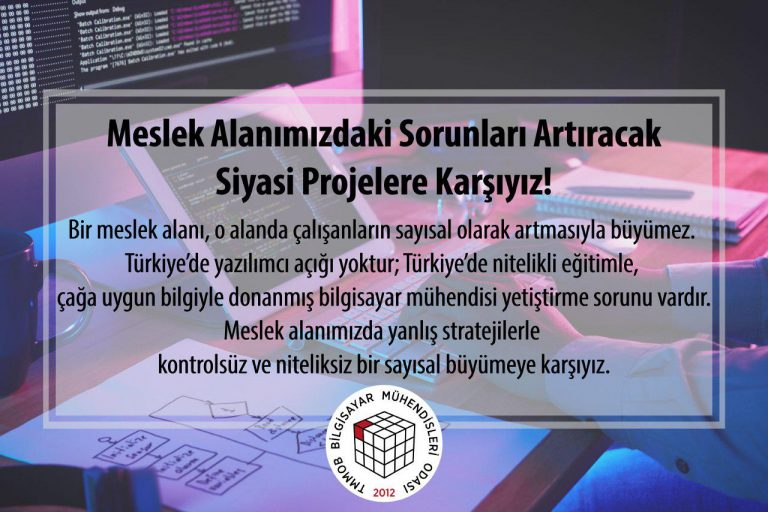
\includegraphics[width=.9\linewidth]{gorseller/bmo-bildiri.jpg}
\end{center}

Yazının tamamını bu konuya ayırmak istemiyorum o yüzden sizleri Bilgisayar
Mühendisleri Odası'nın \href{https://www.bmo.org.tr/2020/04/26/meslek-alanimizdaki-sorunlari-artiracak-siyasi-projelere-karsiyiz/}{bugün yayınladığı bildiriyi okumaya davet ediyorum}.
Bildiride yazılan her şeye ben de sonuna kadar katılıyorum ve destekliyorum.

Bu konu hakkında siz ne düşünüyorsunuz? Yorumlar bölümünde konuşalım.
\section{Tek satırlık kütüphane tüm \href{https://www.zdnet.com/article/another-one-line-npm-package-breaks-the-javascript-ecosystem/}{JavaScript ekosistemini kırdı}}
\label{sec:org886b5a3}
\begin{minted}[breaklines=true,breakanywhere=true,frame=lines, linenos, label=JavaScript]{javascript}
function isPromise(obj) {
  return !!obj &&
    (typeof obj === 'object' || typeof obj === 'function') &&
    typeof obj.then === 'function';
}
\end{minted}

Yukarıdaki tek satırlık fonksiyon aslında \href{https://github.com/then/is-promise}{is-promise} isimli bir JavaScript
kütüphanesi. Yaptığı tek işlem ise verdiğiniz değişkenin "\href{https://developer.mozilla.org/en-US/docs/Web/JavaScript/Reference/Global\_Objects/Promise}{Promise}" objesi olup
olmadığını kontrol etmek ve geriye boolean değer döndürmek. Yaptığı iş bu
kadar basit olmasına rağmen kütüphane(!) olabilmiş, hatta yetmemiş 3.4 milyon
farklı projede kullanılmış, hatta ve hatta komple bir ekosistemi birkaç
saatliğine kırabilmiş. İşte size modern yazılım geliştirme süreçlerindeki
bağımlılık yönetiminin geldiği halin özeti.

Bu kütüphaneye \href{https://github.com/then/is-promise/commit/feb90a40501c8ef69b0c65bdf1eb703182214407}{25 Nisan günü yapılan bir değişiklik} ve \href{https://github.com/then/is-promise/releases/tag/2.2.0}{2.2.0 sürümü}yle
birlikte ES Module desteği gelmişti fakat sanırım bu standardı iyi bir şekilde
projeye eklememiş olacaklar ki sürümün yayınlanmasından sadece birkaç saat
sonra bu kütüphaneyi kullanan projelerin geliştiricileri \href{https://github.com/then/is-promise/issues/12}{hatalar almaya}
\href{https://github.com/then/is-promise/issues/13}{başladılar}. Kütüphanenin yeni sürümündeki hatanın etki alanı oldukça büyük:
Facebook'un "\href{https://github.com/facebook/create-react-app/issues/8896\#issuecomment-619406384}{Create React App}" aracından, Google'ın \href{https://github.com/then/is-promise/issues/23}{AngularJS framework'üne},
oradan Amazon'un AWS Serverless komut satırı aracına kadar birçok yerden
sarsıntılar hissedildi. Hali hazırda çalışan uygulamalarda anlık bir soruna
yol açmadı fakat geliştiriciler derleme sırasında hata aldıkları için
projelerin geliştirilme süreci aksamış oldu.

Neyse ki sorunun çözülmesi fazla uzun sürmedi. Birkaç saat içerisinde önceki
değişiklikleri geri alan ve sorunu çözen 2.2.2 sürümü yayınlandı.

Aslında JavaScript ekosistemi için bu olay hiç de yeni bir şey değil. Takip
edenler mutlaka hatırlayacaktır. 2016 yılında da left-pad isimli bir
kütüphanenin npm'den silinmesi üzerine aynı şeyler yaşanmıştı. Üstelik ilgili
kütüphanenin geliştiricisi Türkiye'den bir isimdi: \href{https://kodfabrik.com/}{Azer Koçulu}. Konuyla ilgili
kendisinin konuk olduğu \href{https://podtail.com/en/podcast/devpod/-036-azer-koculu/}{şöyle bir podcast yayını} var. Mutlaka dinlemenizi
tavsiye ederim.

Görünüşe göre yazılım camiası o olaydan dersini almamış. Bu olay da her ne
kadar \href{https://www.reddit.com/r/programming/comments/g7xweu/another\_1liner\_npm\_package\_broke\_the\_js\_ecosystem/}{Reddit} ve \href{https://news.ycombinator.com/item?id=22979245}{HackerNews} gibi platformlarda uzun süre ilk sıralarda otursa
da yine ders çıkarılacağını pek sanmıyorum. Modern yazılım geliştirme
süreçlerinin geldiği durumu pek beğenmiyorum. Şu yukarıdaki gibi tek satırlık
bir kodu bile üçüncü parti kütüphane olarak eklemek bana soracak olursanız
üşengeçlikten başka bir şey değil.

Bu konu hakkında siz ne düşünüyorsunuz? Günümüz modern yazılım geliştirme
süreçlerinden memnun musunuz? Sizin karşılaştığınız ya da tespit ettiğiniz
sorunlar neler? Yorumlar bölümünde konuşalım.
\section{Hollanda, kamu hizmetlerinin yazılımlarının \href{https://joinup.ec.europa.eu/collection/open-source-observatory-osor/news/legal-barrier-be-removed}{açık kaynak olmasını teşvik etmeye başlayacak}}
\label{sec:org3099054}
Geçtiğimiz hafta Hollanda İçişleri ve Krallık ilişkileri Devlet Sekreteri
Raymond Knops, kamu kurum ve kuruluşlarında açık kaynak kullanımıyla ilgili
\href{https://www.rijksoverheid.nl/documenten/kamerstukken/2020/04/17/kamerbrief-inzake-vrijgeven-broncode-overheidssoftware}{açık mektup yayınlayarak} (metnin İngilizce çevirisi için \href{https://www.reddit.com/r/freesoftware/comments/g77202/netherlands\_commits\_to\_free\_software\_by\_default/fogpeub/}{bu reddit yorumu}na
bakabilirsiniz) diğer ülkelere de çağrıda bulundu.

Metinde kamu kurum ve kuruluşlarının ürettiği yazılımları neden açık kaynak
olarak paylaşılması gerektiğinden bahseden Knops, "Eğer iyi bir nedeniniz
yoksa kamu yazılımlarını açık kaynak olarak paylaşmalısınız" dedi. Tabii ki
bunlara askeri sistemler vb. güvenliğin çok hassas olduğu projeler dahil
değil. Bu bağlamda Hollanda'nın da 2021'in ilk aylarında kamu yazılımlarının
açık kaynak yapılmasını önünde duran bazı yasal bariyerleri kaldıracaklarını
ve kamu kurumlarının yazılımlarının daha şeffaf olması yönünde düzenlemeler
yapacaklarını belirttiler. Fakat bu yeni düzenlemeler çıktığı tarihten sonra
geliştirilmeye başlanan yazılımları kapsayacak görünüyor. Yalnız şunu
belirtmekte fayda var "artık kamu kurum ve kuruluşları yazılımlarını açık
kaynak yapmak zorunda" gibi bir durum yok, şu an sadece kurumlara
yazılımlarını açık kaynak yapabilmeleri için imkan ve teşvik sağlıyorlar.

Bu haber farklı bir kaynakta da karşıma çıktı fakat biraz kendi taraflarına
yormuşlar gibi geliyor bana. Özgür Yazılım Vakfı Avrupa (FSFE) organizasyonun
(bildiğimiz Özgür Yazılım Vakfı ile çalışmaları var fakat birbirlerine bağlı
değiller) web sitesinde de bu haber "\href{https://fsfe.org/news/2020/news-20200424-01.html}{Netherlands commits to Free Software by
default}" başlığıyla yayınlandı. Fakat ben Raymond Knops'un yayınladığı açık
mektupun İngilizce çevirisini okuduğumda özgür yazılımla ilgili bir ibareye
rastlamadım. Knops, daha çok açık kaynağın getirdiği ekonomik ve teknik
faydalardan bahsetmiş. Teknik faydalardan kast ettiğim şunlar: topluluk
tarafından desteklenme, ortak geliştirme yapabilme, diğer geliştiricilerin
katkı sağlayabilmesi, şeffaflık. Burada özgür yazılım tarafına yorabileceğimiz
bir ifade var, o da "şeffaflık". Yazıda parantez içerisinde "açık kaynak"
("open source") ifadesini de kullanmışlar fakat benim bu haberden anladığım
Hollanda da, büyük yazılım firmaları gibi açık kaynağı kendi amaçları için
kullanmak istiyor. Ben de bir özgür yazılım destekçisiyim ama bu habere
tarafsız gözle incelediğimde özgür yazılım adına bir ifade göremedim. Yine de
başlangıç için çok güzel bir gelişme, ileride özgür yazılımı konuşmanın önünü
açabilecek bir gelişme bence.

Bu konu hakkında siz ne düşünüyorsunuz? Sizce kamu kaynakları kullanılarak
oluşturulan yazılımların kaynak kodları yine kamuya açılmalı mı? Devletlerin
özgür yazılım tarafına geçmesi mümkün mü? Yorumlar bölümünde konuşalım.

Ayrıca yeri gelmişken Özgür Yazılım Vakfı Avrupa tarafından başlatılmış
"Halkın Parası. Halkın Kodu!" ("Public Money? Public Code!") kampanyasının da
\href{https://www.youtube.com/watch?v=iuVUzg6x2yo}{şu videosunu izlemenizi öneririm}.
\section{GitHub'ın yeni bildirim sayfası tasarımı \href{https://github.blog/2020-04-22-improving-notifications-for-everyone/}{Beta'dan çıktı}}
\label{sec:org36abec8}
Popüler uzak git sunucularından biri olan GitHub, bu hafta içerisinde uzun bir
süredir Beta programında olan bildirim sayfasının yeniden tasarlanmış halini
program kapsamından çıkararak, herkes tarafından erişilebilir yaptı. Bu yeni
tasarımda artık bildirimler arasında arama yapabilir ve çeşitli filtreler
seçerek ekranınızı özelleştirebilirsiniz.

\begin{figure}[htbp]
\centering
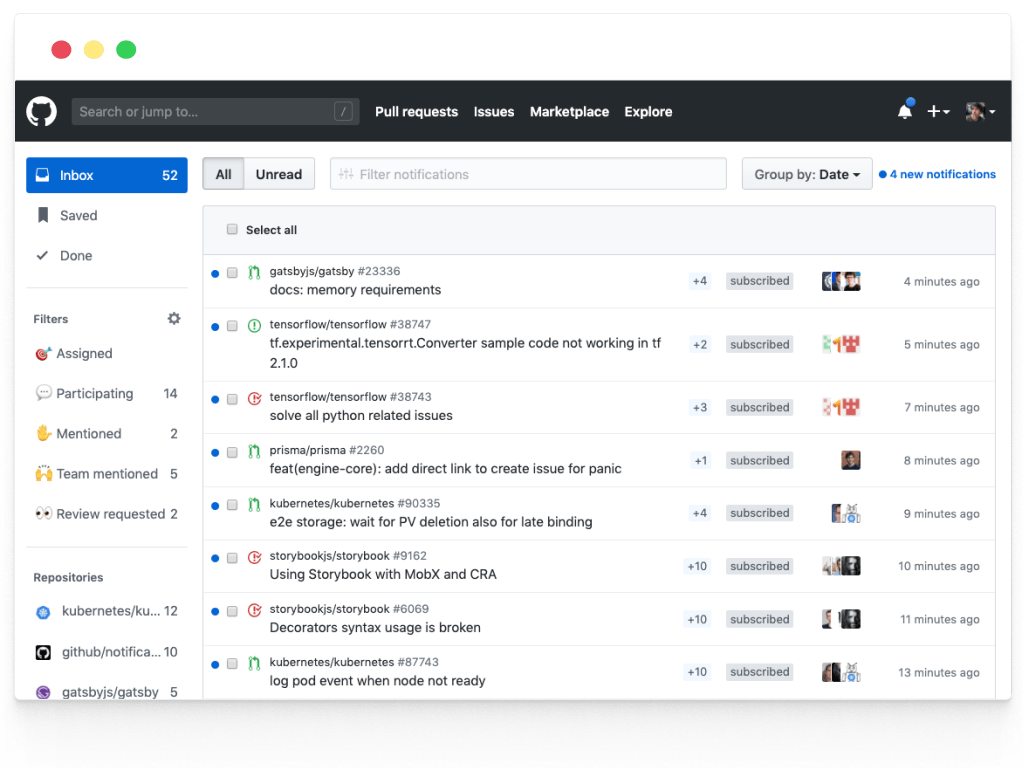
\includegraphics[width=.9\linewidth]{gorseller/github-bildirimler-yeni.png}
\caption{GitHub'ın yeni bildirim sayfası tasarımı}
\end{figure}

Yeni tasarımı incelemek için siz de kendi \href{https://github.com/notifications}{GitHub hesabınızın bildirimler
sayfasına} göz atabilirsiniz.
\section{GitLab \href{https://about.gitlab.com/releases/2020/04/22/gitlab-12-10-released/}{12.10 sürümü yayınlandı}}
\label{sec:org7d5e4c9}
GitHub'ın en büyük rakiplerinden biri olan GitLab, bu hafta içerisinde 12.10
numaralı sürümünü duyurdu. Bu sürümle ile birlikte gelen bazı özellikler
ücretsiz kullanıcılara da açıkken, bazıları da sadece ücretli paketlerdeki
lisanslı kullanıcılara açık. Gelin birkaç özelliği birlikte inceleyelim.

\subsection{CI/CD anahtarlarını HashiCorp Vault üzerinden getirme}
\label{sec:org42ea832}
Artık HashiCorp firması tarafından sağlanan şifre, anahtar ve sertifika
yönetimi servisi Vault üzerinden ihtiyacımız olan anahtarları getirip, CI
(Continuous Integration) ve CD (Continuous Delivery) süreçleri üzerinde JWT
(JSON Web Token) doğrulama yöntemiyle kullanabileceğiz. Bu özelliklik
ücretsiz ve ücretli tüm GitLab kullanıcılarına açık.
\subsection{Jira üzerinden issue'leri içeri aktarma}
\label{sec:orga1a08a4}
Atlassian firması tarafından issue takibi ve proje yönetimi hizmeti olarak
sağlanan Jira platformu üzerindeki issue'leri artık GitLab'a aktarabileceğiz.
Bu özellik de herkesin kullanımına açık.
\subsection{GitHub CI işlerini AWS Fargate üzerinde otomatik ölçekleme}
\label{sec:orgeb4a695}
Günümüz modern yazılım geliştirme süreçlerinin önemli bir parçası da artık
Continuous Integration süreçleri oldu. Projede bir değişiklik yaptığınızda bu
değişikliklerin yol açabileceği şeyler farklı sistemler üzerinde denenmek ve
raporlanmak zorunda. Bu deneme ve raporlama işleri de GitLab tarafında GitLab
CI ile çözülüyor. Bu güncelleme ile birlikte artık CI süreçlerinde çalışan
işler AWS Fargate üzerinde otomatik ölçeklenebilecek (autoscaling).
Dolayısıyla deneme ve raporlama süreçleri daha erken bitebilecek. Bu özelliği
GitLab.com üzerinde kullanamıyorsunuz fakat kendi sunucunuzda GitLab
kullanırken ücretsiz olarak bu özellikten faydalanabiliyorsunuz.

\begin{center}
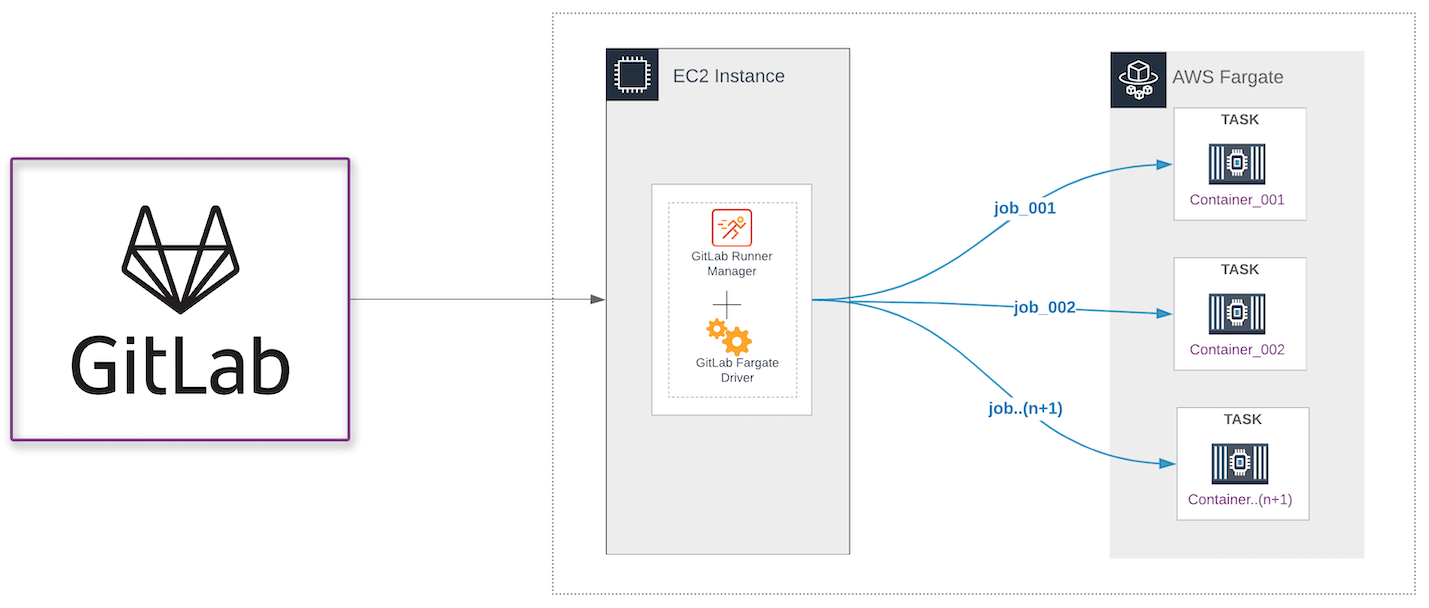
\includegraphics[width=.9\linewidth]{gorseller/gitlab-autoscale-aws.png}
\end{center}

Bu sürüm ile birlikte pek çok farklı özellikte geldi fakat hepsine burada
değinemiyorum. GitLab 12.10 sürümüyle birlikte gelen diğer özellikler için
konu başlığına eklediğim bağlantıya tıklayabilirsiniz.
\section{NodeJS \href{https://medium.com/nodejs/node-js-version-14-available-now-8170d384567e}{14.0 sürümü yayınlandı}}
\label{sec:orgfd2dc34}
Sunucu tarafında JavaScript kullanımına olanak sağlayan NodeJS, bu hafta
itibariyle 14 numaralı sürümünü yayınladı. Bu sürümle birlikte gelen bazı
özelliklere birlikte bakalım.

\begin{figure}[htbp]
\centering
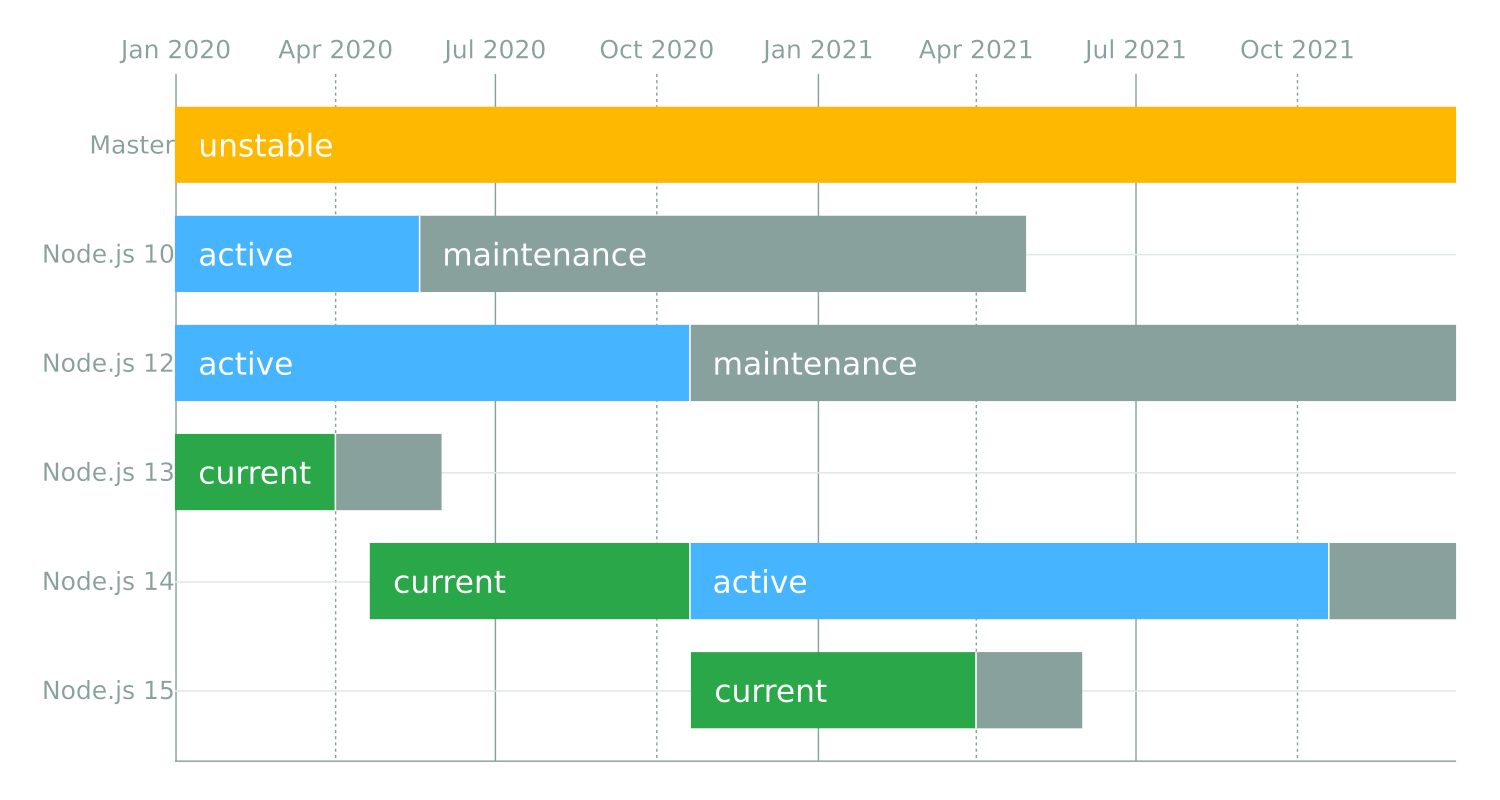
\includegraphics[width=.9\linewidth]{gorseller/node14-surum.png}
\caption{Şu anda "Current" dalında olan bu sürüm Ekim 2020'de Long-Term Support sürecine girecek. Yani üretim ortamında kullandığınız bir NodeJS var ise onu hemen güncellemeniz tavsiye edilmez. Uzun dönem desteklenecek hale geldiğince üretim ortamı için daha uygun olacaktır.}
\end{figure}

\subsection{JavaScript motoru sürümü V8 8.1 olarak güncellendi}
\label{sec:org7bc5b60}
Bu JavaScript motoruyla birlikte gelen bazı özellikler de doğal olarak
NodeJS'e gelmiş oldu. Bunlardan bazıları şu şekilde:

\begin{itemize}
\item \href{https://developer.mozilla.org/en-US/docs/Web/JavaScript/Reference/Operators/Optional\_chaining}{Optional Chanining}
\item \href{https://wiki.developer.mozilla.org/en-US/docs/Web/JavaScript/Reference/Operators/Nullish\_Coalescing\_Operator}{Nullish Coalescing}
\item \href{https://developer.mozilla.org/en-US/docs/Web/JavaScript/Reference/Global\_Objects/Intl/DisplayNames}{Intl.DisplayNames}
\item \texttt{calendar} ve \texttt{numberingSystem} seçenekleri \href{https://developer.mozilla.org/en-US/docs/Web/JavaScript/Reference/Global\_Objects/Intl/DateTimeFormat}{Intl.DateTimeFormat} için
aktifleştirildi.
\end{itemize}
\subsection{\href{https://nodejs.org/api/async\_hooks.html\#async\_hooks\_class\_asynclocalstorage}{Deneysel Asenkron Local Storage API}}
\label{sec:orgb69f7f7}
Asenkron yapılar artık günümüzde birçok projede kullanılıyor. Kısaca
açıklamak gerekirse bu yapılar sayesinde belirli bir zaman alan işlemlerin
yazılımı durdurmasının önüne geçiliyor. Yani siz bir siteye girdiğinizde,
sitenin içerisindeki bazı bilgiler başka servislerden geliyor olabilir. Bu
bilgilerin gelme işlemi devam ederken siz site üzerinde gezinti yapmaya devam
edebiliyorsunuz. İşte bu yapı artık Local Storage için de geldi. Artık Local
Storage üzerine veri kayıt ederken ve okurken asenkron olabileceğiz.


NodeJS 14 ile birlikte gelen diğer özellik ve değişiklikler için konu
başlığına eklediğim bağlantıya; değindiğim özelliklerin detayları için de
ilgili alt başlığın içerisindeki bağlantılara tıklayabilirsiniz. Ayrıca
alternatif kaynak için IBM'deki geliştiriciler tarafından hazırlanmış \href{https://www.youtube.com/watch?v=2iIJhi6\_ngo}{şu
videoyu da izleyebilirsiniz}.
\section{Python 2 için \href{https://www.python.org/downloads/release/python-2718/}{son güncelleme: 2.7.18}}
\label{sec:org25a1836}
Geçtiğimiz senenin eylül ayı içerisinde Python 2 sürüm dalının 3 aylık ömrü
kaldığını haber vermiştim (bkz: \href{../../2019/yazilim-gundemi-09.pdf}{Yazılım Gündemi - 9}). Bu hafta ise Python 2
sürüm dalı son güncellemesini aldı. Artık Python 2 sürümü geliştirilmeye devam
edilmeyecek. Bu haber vesilesiyle Python 2 ile artık yeni projelere
başlanmamasını, var olan aktif geliştirilen projelerin de Python 3 sürüm
dalına geçirilmesini tavsiye etmiş olayım.

Ayrıca konuyla ilgili StackOverflow'un Blog sayfasında da \href{https://stackoverflow.blog/2020/04/23/the-final-python-2-release-marks-the-end-of-an-era/}{bir yazı yayınlandı}.
İlgili arkadaşlar nostalji yapmak için o yazıyı da okuyabilirler.
\newpage
\section{Yaklaşan Online Etkinlikler \#EvdeKal}
\label{sec:org9ae10b2}
\begin{longtable}{|p{9.5cm}|l|}
\hline
Etkinlik İsmi & Tarihi\\
\hline
\endfirsthead
\multicolumn{2}{l}{Önceki sayfadan devam ediyor} \\
\hline

Etkinlik İsmi & Tarihi \\

\hline
\endhead
\hline\multicolumn{2}{r}{Devamı sonraki sayfada} \\
\endfoot
\endlastfoot
\hline
\href{https://kommunity.com/tracikkaynak/events/acik-seminer-11-gun-ml-algorithms-use-cases-watson-studio-workshops-hands-on-8936cb51}{AçıkSeminer 11. Gün: Makine Öğrenmesine Giriş} & 29 Nisan 14:00\\
\href{https://kommunity.com/akademi/events/carbon-black-uzerinden-olay-mudahalesi-ve-tehdit-avciligi-c4276138}{Carbon Black Üzerinden Olay Müdahalesi ve Tehdit Avcılığı} & 29 Nisan 16:30\\
\href{https://kommunity.com/mavidurakio/events/s1e38-yazilimci-bulusmasi-3c624265}{Yazılımcı Buluşması (MaviDurak-IO)} & 29 Nisan 20:45\\
\href{https://kommunity.com/kadin-yazilim-tasarim/events/soylesi-kadin-yazilimcilar-toplaniyor-yazilima-adim-atmak-canli-yayin-a2709f1b}{Kadın Yazılımcılar Toplanıyor - Yazılıma Adım Atmak} & 29 Nisan 21:00\\
\href{https://kommunity.com/istanbulphp/events/4x4-laravel-a5e89ab9}{4x4 Laravel} & 29 Nisan 21:00\\
\href{https://kommunity.com/devops-turkiye/events/kubernetes-insights-with-humio-3f940956}{Kubernetes insights with Humio} & 29 Nisan 22:00\\
\href{https://kommunity.com/tracikkaynak/events/acik-seminer-12-gun-dijital-cagda-deneyim-yonetimi-50cbfc05}{AçıkSeminer 12. Gün: Dijital Çağda Deneyim Yönetimi} & 30 Nisan 14:00\\
\href{https://kommunity.com/mobilerdev/events/fluttera-dogru-2-dart-fecaa463}{Flutter'a Doğru no.2 - Dart} & 30 Nisan 21:00\\
\href{https://kommunity.com/cloud-and-serverless-turkey/events/ramazan-ozel-2-nosql-nedir-ve-ne-zaman-kullanilmali-0e8533fb}{NoSQL nedir ve ne zaman kullanılmalı} & 30 Nisan 23:00\\
\href{https://kommunity.com/tracikkaynak/events/acik-seminer-13-gun-acik-kaynak-kodlu-veri-bilimi-yaklasim-0a14d5dd}{AçıkSeminer 13. Gün: Açık Kaynak Veri Bilimi} & 1 Mayıs 14:00\\
\href{https://kommunity.com/react-native-turkey/events/etkinlik-iki-aws-amplify-ve-react-1735e369}{ReactJS ve AWS Amplify - Serverless Web Development} & 1 Mayıs 16:10\\
\href{https://kommunity.com/akademi/events/bulutta-siber-olay-mudahalesi-b92d1d73}{Bulut'ta Siber Olay Müdahalesi} & 1 Mayıs 16:30\\
\href{https://kommunity.com/flutter-izmir-1/events/flutter-izmir-canli-yayini-2-f1b24bbf}{Flutter İzmir Canlı Yayını - 2} & 2 Mayıs 13:00\\
\href{https://kommunity.com/cloud-and-serverless-turkey/events/kubernetes-hands-on-1-kubernetes-installation-the-hard-way-7bf5e75f}{Kubernetes Installation, The Hard Way} & 2 Mayıs 13:30\\
\href{https://kommunity.com/tensorflow-turkey/events/ml-in-the-wild-series-1-data-preparation-73ac8e24}{ML in the Wild Series - 1: Data Preparation} & 2 Mayıs 21:00\\
\href{https://kommunity.com/devnot-yazilimci-bulusmalari/events/fluttera-giris-e38503c7}{Flutter'a Giriş} & 2 Mayıs 22:00\\
\href{https://kommunity.com/teknolojisohbetleri/events/elasticsearch-ve-kibana-21cec45e}{Elasticsearch ve Kibana} & 3 Mayıs 21:00\\
\href{https://kommunity.com/cloud-and-serverless-turkey/events/ramazan-ozel-3-kim-on-call-olmali-neden-ve-nasil-24a94df1}{Kim On-Call olmalı, neden ve nasıl} & 3 Mayıs 23:00\\
\hline
\end{longtable}
\section{Diğer Haberler}
\label{sec:orga73d719}
\begin{itemize}
\item OpenSSL'deki kritik bir \href{https://www.openssl.org/news/secadv/20200421.txt}{güvenlik açığı kapatıldı}.
\item BitBucket, COVID-19 salgını yüzünden Mercurial kullanan \href{https://bitbucket.org/blog/sunsetting-mercurial-support-in-bitbucket}{depoları silmeyi
erteledi}. Son gün: 1 Temmuz 2020. (bkz: \href{../../2019/06/yazilim-gundemi-06.pdf}{Yazılım Gündemi - 6})
\item Amazon Web Services, Afrika'da (Cape Town) \href{https://aws.amazon.com/blogs/aws/now-open-aws-africa-cape-town-region/}{veri merkezi açtı}: \texttt{af-south-1}.
\item AWS ChatBot, Beta \href{https://aws.amazon.com/blogs/aws/aws-chatbot-chatops-for-slack-and-chime/}{programından çıktı}.
\item Google, Anthos \href{https://cloud.google.com/blog/topics/anthos/anthos-for-aws-is-now-ga}{platformunu genişletiyor}.
\item Facebook ve Amazon yeni ortak PyTorch \href{https://aws.amazon.com/blogs/aws/announcing-torchserve-an-open-source-model-server-for-pytorch/}{araçlarını duyurdular}: \href{https://github.com/pytorch/serve}{TorchServe},
\href{https://ai.facebook.com/blog/facebook-ai-aws-partner-to-release-new-pytorch-libraries-/}{Alternatif}
\item PyTorch \href{https://pytorch.org/blog/pytorch-1-dot-5-released-with-new-and-updated-apis/}{1.5 sürümü yayınlandı}.
\item ProtonMail Android uygulaması \href{https://protonmail.com/blog/android-open-source/}{açık kaynak oldu}.
\item Android 11 Geliştirici \href{https://android-developers.googleblog.com/2020/04/android-11-developer-preview-3.html}{Ön İzlemesi 3 sürümü yayınlandı}.
\item .NET 5.0 \href{https://devblogs.microsoft.com/dotnet/announcing-net-5-0-preview-3/}{Preview 3 sürümü duyuruldu}.
\item Windows Terminal Preview \href{https://devblogs.microsoft.com/commandline/windows-terminal-preview-v0-11-release/}{v0.11 sürümü yayınlandı}.
\item Go Geliştirici Anketi 2019 \href{https://blog.golang.org/survey2019-results}{sonuçları açıklandı}.
\item Rust programlama dilinin \href{https://blog.rust-lang.org/2020/04/23/Rust-1.43.0.html}{1.43.0 sürümü yayınlandı}.
\item R programlama dilinin \href{https://stat.ethz.ch/pipermail/r-announce/2020/000653.html}{4.0.0 sürümü yayınlandı}.
\item VueJS v3.0.0 \href{https://github.com/vuejs/vue-next/releases/tag/v3.0.0-beta.4}{Beta 4 sürümü yayınlandı}.
\item Angular \href{https://github.com/angular/angular/releases/tag/9.1.3}{9.1.3 sürümü yayınlandı}.
\item ClojureScript \href{https://clojurescript.org/news/2020-04-24-release}{1.10.741 sürümü yayınlandı}.
\item Embeddable Common-Lisp \href{https://common-lisp.net/project/ecl/posts/ECL-20424-release.html}{20.4.24 sürümü yayınlandı}.
\item TestContainers Java kütüphanesinin \href{https://github.com/testcontainers/testcontainers-java/releases/tag/1.14.1}{1.41.1 sürümü yayınlandı}.
\item WineHQ \href{https://www.winehq.org/announce/5.7}{5.7 sürümü yayınlandı}.
\item css.gg \href{https://github.com/astrit/css.gg/releases/tag/2.0.0}{v2.0.0 çıktı}.
\item Blitz \href{https://github.com/blitz-js/blitz/releases/tag/v0.6.6}{v0.6.6 çıktı}.
\item DataFusion \href{https://andygrove.io/2020/04/datafusion-0.17.0/}{v0.17.0 çıktı}.
\item Tide \href{https://github.com/http-rs/tide/releases/tag/v0.8.0}{v0.8.0 çıktı}.
\item i18n-ally \href{https://github.com/antfu/i18n-ally/releases/tag/v2.0.3}{v2.0.3 çıktı}.
\item Cap'n Proto \href{https://capnproto.org/news/2020-04-23-capnproto-0.8.html}{v0.8 çıktı}.
\item Voyager \href{https://github.com/appscode/voyager/releases/tag/v12.0.0-rc.2}{v12.0.0-rc.2 çıktı}.
\end{itemize}
\section{Lisans}
\label{sec:orge8e9961}
\begin{center}
\begin{center}

\includegraphics[height=1.5cm]{../../../img/CC_BY-NC-SA_4.0.png}
\end{center}

\href{yazilim-gundemi-2020-16.pdf}{Yazılım Gündemi - 2020/16} yazısı \href{https://erenhatirnaz.github.io}{Eren Hatırnaz} tarafından \href{http://creativecommons.org/licenses/by-nc-sa/4.0/}{Creative Commons
Atıf-GayriTicari-AynıLisanslaPaylaş 4.0 Uluslararası Lisansı} (CC BY-NC-SA 4.0)
ile lisanslanmıştır.
\end{center}
\end{document}
